Generally, finding more learning resources can be broken down into having a particular problem you are trying to solve, and learning what is possible with a package.
\section{Specific problems}
It is very likely someone else had the same exact problem you had, so use your preferred search engine!
Invariably you will run into \href{https://tex.stackexchange.com/}{Stack Exchange}, and adapting these solutions to your exact needs is a really important skill.

Some times you will find particularly well detailed solutions, like this \href{https://tex.stackexchange.com/questions/604496/how-to-generate-beautiful-tables-in-latex}{one} explaining how to produce beautiful tables.
Most likely, however, you will find a lot of options and commands you may not understand, like \href{https://tex.stackexchange.com/questions/603781/how-can-i-draw-the-following-graph-with-tikz}{this}.
In that case, the package documentation is key.
\section{Package information}
If you know what you are looking for, package documentation can be found on \href{https://www.ctan.org/pkg/}{CTAN}.
And if you are using VSCode, clicking on the package's name will give you a link to the documentation:
\begin{figure}[h]
\centering
    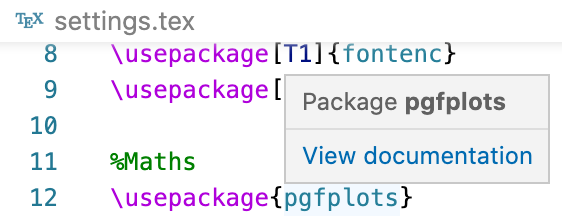
\includegraphics[width=0.5\textwidth]{figures/package-info.png}
\caption{Viewing package documentation from inside VSCode}
\end{figure}

You may find documentation that includes examples, such as \href{https://anorien.csc.warwick.ac.uk/mirrors/CTAN/graphics/pgf/contrib/pgfplots/doc/pgfplots.pdf}{\texttt{pgfplots}}, or general explanations about best practices, like \href{https://mirror.ox.ac.uk/sites/ctan.org/macros/latex/contrib/booktabs/booktabs.pdf}{\texttt{booktabs}}.
For the latter, it is likely someone has detailed explanations of a use-case in Stack Exchange.